\chapter{Kiến trúc Pipeline, Hiện thực và Kiểm thử}
\label{ch:kientruc_pipeline}

\section{Kiến trúc Tổng thể 5 Phân vùng}
Hệ thống được thiết kế theo mô hình đường ống khép kín gồm \textbf{5 phân vùng liên thông} (Hình~\ref{fig:arch_5zones}): (1) \textit{Upstream Data Sources}, (2) \textit{AWS Serverless \& Terraform IaC}, (3) \textit{Databricks Lakehouse Medallion}, (4) \textit{BI Serving \& Analytics (QuickSight + Streamlit 5 trang)}, và (5) \textit{ML Demand Forecasting \& XAI} bàn giao precomputed artifacts trực tiếp cho Trang 5 của Dashboard.

\begin{figure}[H]
\centering
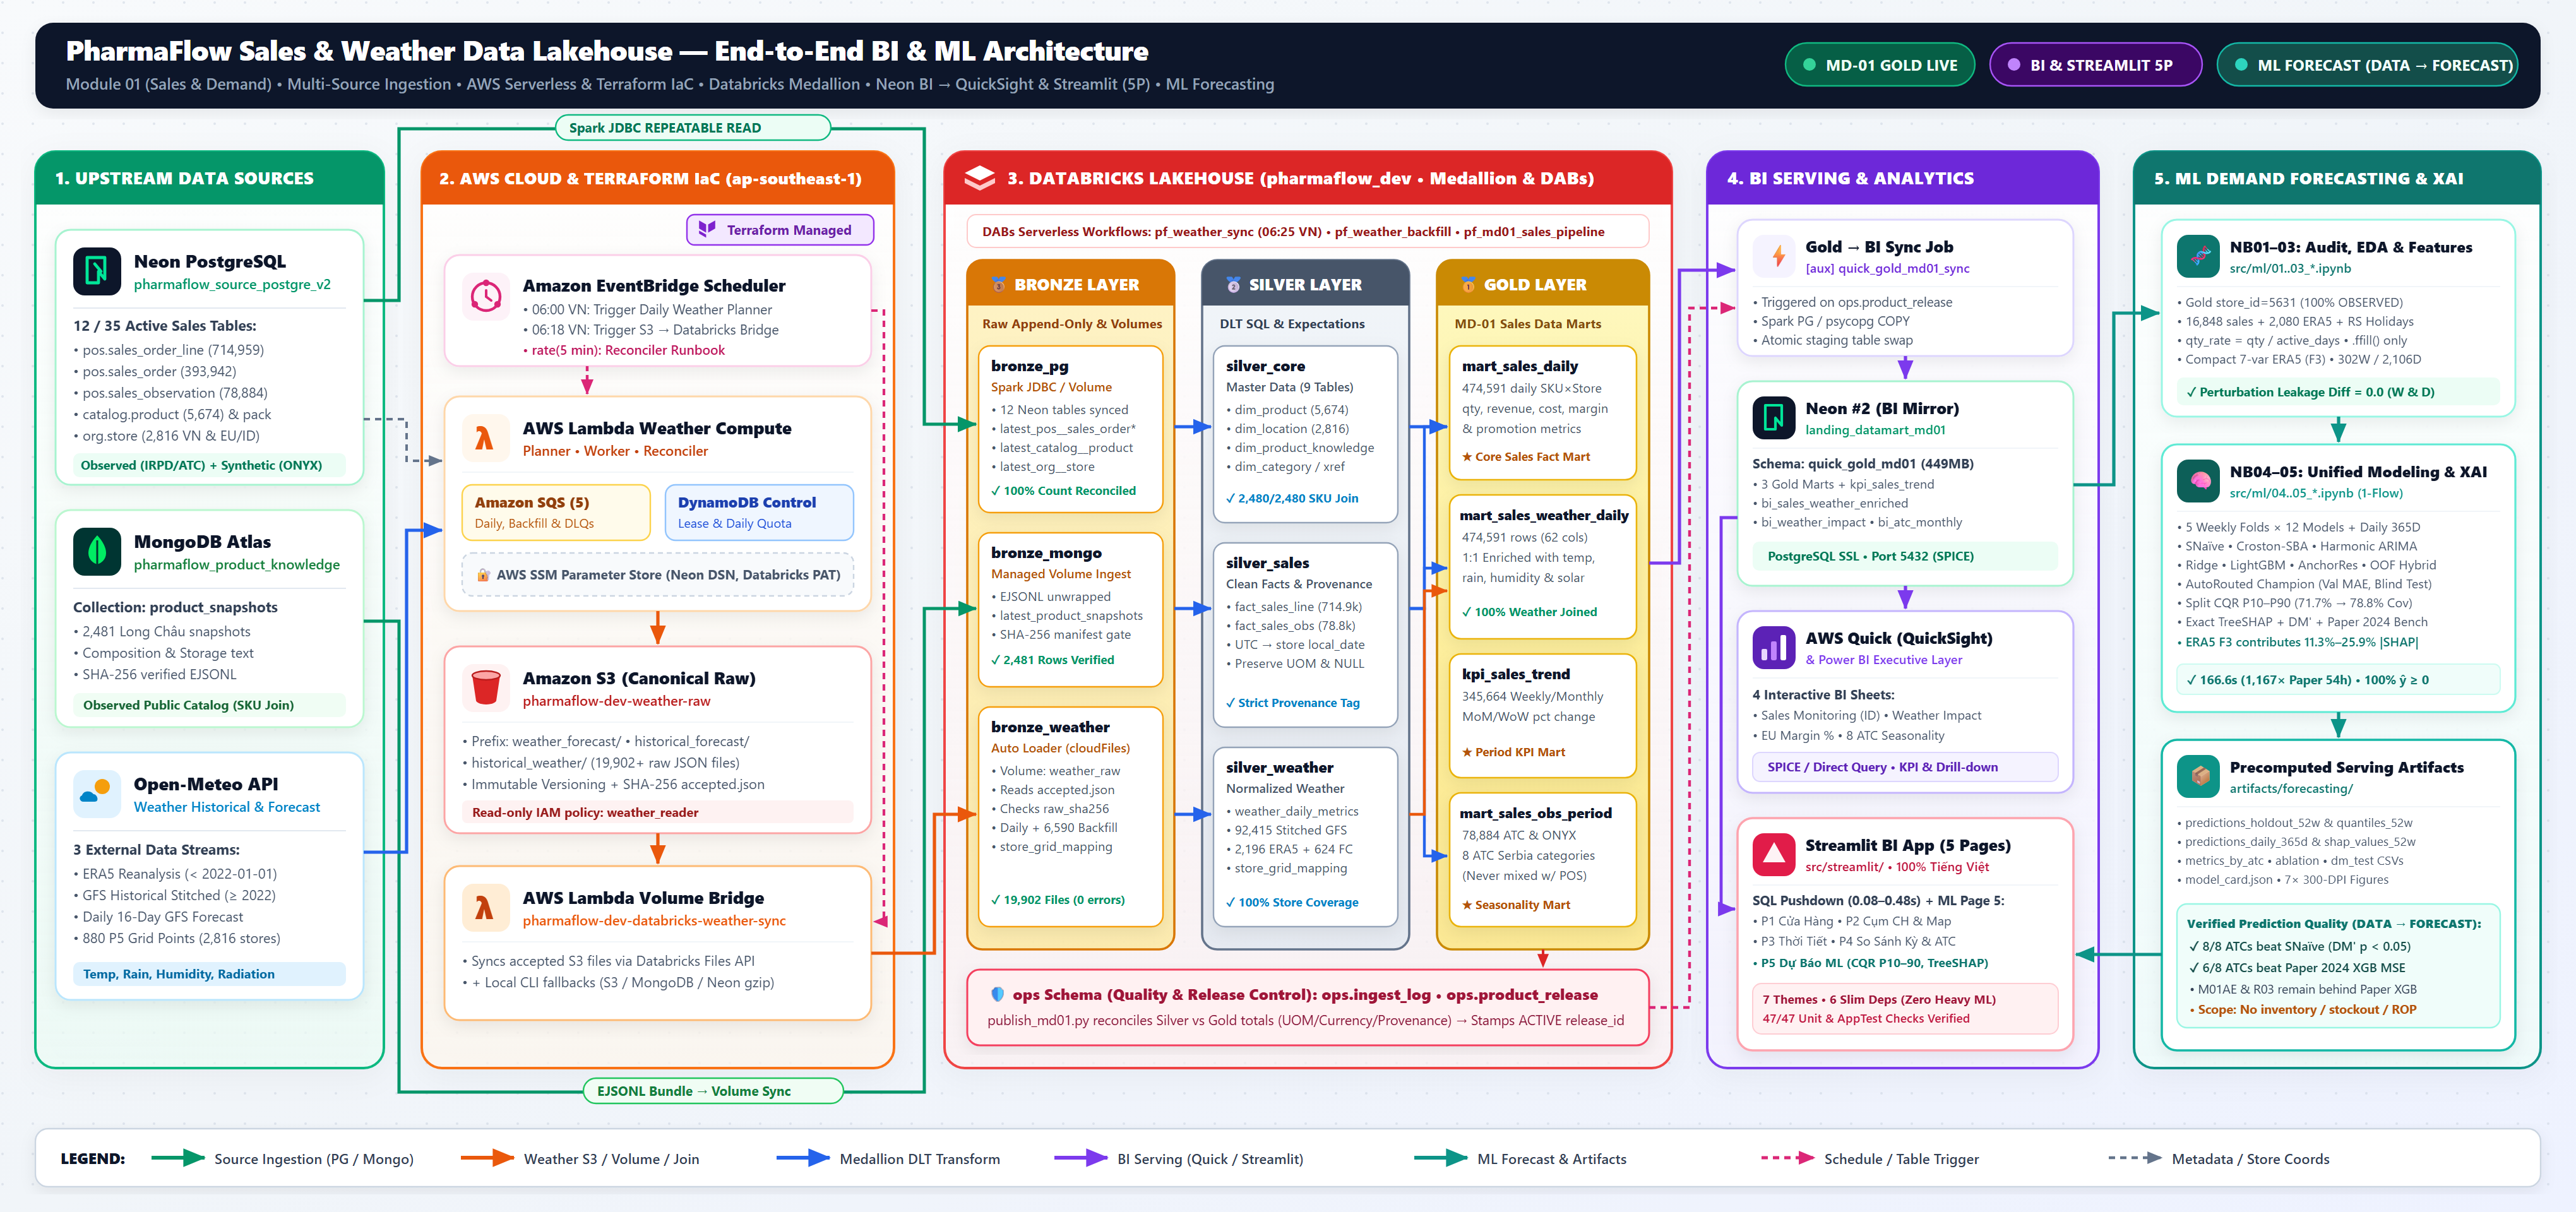
\includegraphics[width=\textwidth]{../images/pharmaflow-sales-bi-architecture.png}
\caption{Kiến trúc tổng thể 5 phân vùng của hệ thống PharmaFlow Sales, Weather Lakehouse, BI và ML Forecasting}
\label{fig:arch_5zones}
\end{figure}

\section{Chi tiết Hiện thực Các Tầng Kỹ thuật}
\subsection{Tầng Thu thập Đám mây (AWS Serverless \& Terraform IaC)}
Toàn bộ hạ tầng vùng \texttt{ap-southeast-1} được khai báo bằng mã nguồn \textbf{Terraform} (\texttt{src/infra/terrafrom/}): Amazon EventBridge lập lịch \texttt{06:00 VN} kích hoạt Lambda Planner chia cụm \texttt{880} điểm lưới \texttt{0.111$^\circ$} đẩy vào \texttt{5} hàng đợi SQS; Lambda Worker kiểm soát hạn mức bằng DynamoDB và ghi tệp thô vào S3 kèm checksum SHA-256; \texttt{06:18 VN} Lambda Volume Bridge đồng bộ tệp mới sang Databricks Managed Volume qua Files API.

\subsection{Tầng Lakehouse (Databricks Asset Bundles \& DLT)}
Triển khai qua Databricks Asset Bundles (\texttt{databricks.yml}, Serverless trên Free Edition \texttt{pharmaflow\_dev}):
\begin{itemize}[leftmargin=1.5em]
  \item \textbf{Bronze:} Spark JDBC (\texttt{REPEATABLE READ}) kéo 12/35 bảng hoạt động từ Neon PostgreSQL; đọc EJSONL MongoDB khớp \texttt{2,480/2,480} SKU; Auto Loader nạp \texttt{19,902} tệp thời tiết kiểm chứng \texttt{raw\_sha256} với \texttt{0} lỗi.
  \item \textbf{Silver (\texttt{DLT SQL}):} Chuẩn hóa 9 bảng Master Data (\texttt{silver\_core}), dữ liệu bán hàng tách biệt grain (\texttt{silver\_sales}) và \texttt{95,235} dòng thời tiết ngày (\texttt{silver\_weather}).
  \item \textbf{Gold (\texttt{MD-01}):} Xuất \texttt{mart\_sales\_daily} (\texttt{474,591}), \texttt{mart\_sales\_weather\_daily} (\texttt{474,591}, \texttt{100\%} phủ thời tiết), \texttt{kpi\_sales\_trend} (\texttt{345,664}) và \texttt{mart\_sales\_observation\_period} (\texttt{78,884}). Cổng \texttt{publish\_md01.py} đối soát tổng doanh thu, sản lượng, UOM giữa Silver--Gold trước khi đóng dấu \texttt{ops.product\_release}.
  \item \textbf{BI Serving Bridge (\texttt{src/sync\_quick/}):} Đồng bộ atomic staging table swap sang Neon \#2 (\texttt{quick\_gold\_md01}, \texttt{449 MB}) cùng 3 Analytical Views (\texttt{bi\_sales\_weather\_enriched}, \texttt{bi\_weather\_impact\_summary}, \texttt{bi\_atc\_category\_monthly}).
\end{itemize}

\subsection{Pipeline ML Dự báo Nhu cầu Thống nhất (5 Notebooks: \texttt{01 $\rightarrow$ 05})}
Mã nguồn ML nằm tại \texttt{src/ml/01..05\_*.ipynb}, kết nối 1 luồng thống nhất qua các mốc:
\begin{enumerate}[leftmargin=1.5em]
  \item \textbf{\texttt{NB01} Thu thập \& Kiểm chứng (\textit{Collection}):} Tách kết nối DB chỉ ở bước 1; lưu snapshot \texttt{.parquet} và \texttt{data\_manifest.json}.
  \item \textbf{\texttt{NB02} EDA \& Chẩn đoán Thống kê:} Tính \texttt{ADI / CV$^2$}, \texttt{ADF/KPSS}, \texttt{Ljung-Box}, \texttt{Mann-Kendall}, \texttt{Shapiro-Wilk}, \texttt{STL} và \texttt{CCF} thời tiết cho 8 nhóm ATC.
  \item \textbf{\texttt{NB03} Tiền xử lý \& Chống Rò rỉ:} Chuẩn hóa \texttt{qty\_rate}, xây dựng 3 tầng đặc trưng: \texttt{F1} (14 biến nội sinh trễ/trượt \texttt{.shift(1)}), \texttt{F2} (8 biến lịch/tỷ trọng), \texttt{F3} (cụm 7 biến ERA5 trực giao vật lý: \texttt{temp\_mean}, \texttt{hdd}, \texttt{humidity\_mean}, \texttt{daylight\_duration\_s}, \texttt{temp\_shock\_2w}, \texttt{temp\_mean\_lag1}, \texttt{humidity\_mean\_lag1}).
  \item \textbf{\texttt{NB04} Backtest Thống nhất, CQR \& TreeSHAP:} Đánh giá 12 mô hình qua 5 fold tuần (\texttt{holdout\_52w} + 4 rolling folds) và \texttt{Daily 365D}; xây dựng \textit{Expanding-Block OOF Hybrid} (refit mỗi 26 tuần + \texttt{1\% Val Guard}); định tuyến \texttt{AutoRouted\_Champion} mù Test theo Validation MAE; hiệu chuẩn khoảng tin cậy \textbf{Split CQR} ($P_{10}$--$P_{90}$) và trích xuất chính xác \texttt{TreeSHAP}.
  \item \textbf{\texttt{NB05} Đánh giá \& Đóng gói Serving:} Kiểm định \texttt{DM'}, phân tích độ nhạy \texttt{51W vs 52W}, đối sánh 2 tầng Paper 2024 và xuất \texttt{model\_card.json} phục vụ Trang 5 Streamlit.
\end{enumerate}

\section{Tổng hợp Kết quả Kiểm thử Tự động}
Toàn bộ các phân hệ đều có bộ kiểm thử tự động chạy offline (không phụ thuộc cloud), tóm tắt tại Bảng~\ref{tab:testing_summary}.

\begin{table}[H]
\centering
\caption{Kết quả kiểm thử tự động và kiểm toán chống rò rỉ trên các phân hệ PharmaFlow}
\label{tab:testing_summary}
\renewcommand{\arraystretch}{1.22}
\begin{tabularx}{\textwidth}{|p{0.27\textwidth}|c|p{0.18\textwidth}|X|}
\hline
\textbf{Phân hệ kiểm thử} & \textbf{Số ca} & \textbf{Trạng thái} & \textbf{Phạm vi kiểm chứng chính} \\
\hline
Weather Ingestion (\texttt{tests/weather/}) & \texttt{142} & Đạt (\texttt{142/142}) & Planner, Worker, quota DynamoDB, S3 SHA-256, lưới P5, Reconciler. \\
\hline
Dashboard Streamlit (\texttt{tests/test\_streamlit\_dashboard.py}) & \texttt{47} & Đạt (\texttt{47/47}) & Logic tăng trưởng MoM, khóa đa ĐVT, cấm \texttt{order\_count} cộng sai, AppTest 5 trang qua 3 tracks (\texttt{ONYX}, \texttt{IRPD}, \texttt{Serbia}), slim \texttt{requirements.txt}, kiểm thử Trang 5 \texttt{TreeSHAP}/CQR. \\
\hline
Databricks Pipeline (\texttt{src/pipeline/databricks/tests/}) & \texttt{17} & Đạt (\texttt{17/17}) & Bronze/Silver/Gold SQL logic, sanitization, cổng đối soát \texttt{publish\_md01}. \\
\hline
BI Sync Bridge (\texttt{src/sync\_quick/test\_sync\_quick.py}) & \texttt{6} & Đạt (\texttt{6/6}) & Staging atomic swap và kiểm tra schema 3 BI Helper Views. \\
\hline
Perturbation Leakage Test (\texttt{NB03}) & \texttt{2} (W \& D) & \texttt{max\_diff = 0.0} & Phóng đại dữ liệu Test lên \texttt{99$\times$}, xác nhận mọi đặc trưng Train/Val bất biến tuyệt đối trên cả Weekly (\texttt{302W}) và Daily (\texttt{2,106D}). \\
\hline
\end{tabularx}
\end{table}
